\section{Linemod template matching}
Template matching has always been an attractive approach to computer vision,
especially for real-time applications; some of the main reasons for this
include ease of generalization of
these algorithms (several shapes can be associated to the same object), and
variety of applications (from rigid object detection -- like in this project --
to face recognition); another great advantage over other recognition methods,
such as neural networks, is the need of a relatively simple and fast training phase:
statistics-based methods, in turn, usually require a huge amount 
of samples to be given for evaluation. Usage of template matching also opens
the possibility of starting with a small, offline-generated template database, and training the
objects to be recognized \emph{online}, i.e. acquiring new samples while
recognizing them. In this sense, template matching offers both the benefits of
a fast, model-based training stage and the benefits deriving from
machine-learning algorithms, improving their performance the more they operate.

Two usual problems often come with template-based solutions: the first is that,
as a template usually consists of a set of features to be searched into the
target image, the high-number of templates (even for a relatively small
database) makes this technique come with an extremely high computational cost;
on the other hand, statistical methods require a much longer training phase but
usually base themselves, at recognition time, on a well-defined, very small set of
data (e.g. hue histograms, network coefficients) which is not proportional to the number of elements
analyzed during training phase. Also, template matching usually has poor
results when the analyzed object has little texturing information, as a low
number of features (\emph{keypoints}) can be extracted for each datum.

The Line-MOD template matching algorithm was introduced in 2011 by
Hintestoi{\ss}er, S. et al. (\cite{linemod-paper}) as a way to address these
two problems of template matching approaches. It is based on a previous work by
the same authors, \cite{linemod-origins}, in which the LINE algorithm was
descripted, which solved both the problem of template matching velocity and
texture-less detection, modified to give increased robustness and detection
rates. Another, following work is described in details in sec.
\ref{sec:linemod-pipeline}, and focuses on a practical application of these
algorithms, which is the one to which the system proposed into this project has
inspired.

In this section, this algorithm is explained in detail. Its key concepts are
introduced first, such the concept of image gradient (sec.
\ref{sec:linemod-gradient}) and depth normal computation (sec.
\ref{sec:linemod-depth}). Then, the modality of data representation, which is
the main reason for this algorithm's good performance, is shown in sec.
\ref{sec:linemod-binary}, and finally the algorithm's operating principle is
detailed in sec. \ref{sec:linemod-usage}.

\subsection{Gradient orientation of images} \label{sec:linemod-gradient}
In order to efficiently detect matches into a non-textured image, which is one
of the problems which Line-MOD proposes to solve, a good metric that can be
used for defining salient features into the image is the value (and direction)
of the image \emph{gradient} $\vec{\nabla} (u,v)$ for each pixel. This vector
quantity is defined just like the discrete gradient for a function on the
domain $N$ of natural numbers: by quantizing the differential operator, the
discrete derivate of a function $f(x)$ is given by

\begin{equation}
\frac{df(x)}{dx}=f(x+1)-f(x)
\end{equation}

At the same way, an image can be seen as a set of  functions (one for each
channel) of two variables $(u,v)$, returning the corresponding pixel value at
the desired coordinate, for the desired channel. Thus, a partial, discrete
derivative can be computed onto this function, and the gradient can be defined
as usual as the vector of partial derivatives:

\begin{eqnarray}
\frac{\partial f(u,v)}{\partial u} & = & f(u+1,v)-f(u,v) \\
\frac{\partial f(u,v)}{\partial v} & = & f(u,v+1)-f(u,v) \\
\nabla f(u,v) = \begin{pmatrix} \frac{\partial f(u,v)}{\partial u} \\
\frac{\partial f(u,v)}{\partial v} \end{pmatrix} & = &
\begin{pmatrix}f(u+1,v)\\ f(u,v+1)\end{pmatrix}-\begin{pmatrix}f(u,v) \\
f(u,v)\end{pmatrix}
\end{eqnarray}

This is, anyway, an informal definition, which neverthless finds its
application being simple to implement and computationally cheap. More formal
definitions exist, such the \emph{Sobel operator}, which instead of scanning the
image for difference into a single direction linearly approximates the image as
a continuous function -- it assumes, in fact, that the underlying intensity
function for each channel is continuous
and sampled only in correspondance of pixels' coordinates -- , and thus makes
uses of a convolution operator to approximate samples of the continuous
gradient $G(f)$:

\begin{eqnarray}
  G_x(f) &=& \begin{pmatrix} 
      -1 & 0 & 1 \\
      -2 & 0 & 2 \\
      -1 & 0 & 1 \end{pmatrix}
  \ast f \\
  G\_y(f) &=& \begin{pmatrix} 
      -1 & -2 & -1 \\
      0 & 0 & 0 \\
      1 & 2 & 1 \end{pmatrix}
  \ast f  \\
  G(f) & = & \begin{pmatrix} G_x \\ G_y \end{pmatrix}
\end{eqnarray}

Here, the $\ast$ operator represents convolution of a $3\times 3$ matrix $K$, called
\emph{kernel}, with another matrix $A$: after extending $A$ with a row of $0$ on
each of its four sides, the value of $K\ast A$ is defined for each coordinate
$(u,v)$ as:
\begin{equation}
  (K \ast A)_{u,v} = \text{sum}\begin{pmatrix}
    K_{0,0}A_{u-1,v-1} & 
    K_{0,1}A_{u,v-1} & 
    K_{0,2}A_{u+1,v-1} \\ 
    K_{1,0}A_{u-1,v} & 
    K_{1,1}A_{u,v} & 
    K_{1,2}A_{u+1,v} \\ 
    K_{2,0}A_{u-1,v+1} & 
    K_{2,1}A_{u,v+1} & 
    K_{2,2}A_{u+1,v+1}  
  \end{pmatrix}
\end{equation}

Depending on how the gradient of the image is approximated, the result could
slightly change. However, the intuitive concept is always the same. As an
example, the result of the application of Sobel operator $G$ on a reference
image\footnote{Image taken from the USC SIPI database
  ( http://sipi.usc.edu/database/ ), one of the most common computer vision reference
databases. Original source is unknown.}
 is shown in fig.\ref{fig:scimmia}.

\begin{figure}[htbp]
\centering
\begin{tabular}{c|c}
  \multicolumn{2}{c}{\adjustbox{valign=m}{\includegraphics[height=2in]{./Graphics/scimmia}}}
    \\
    \multicolumn{2}{c}{\vspace{0.2in}} \\
  \adjustbox{valign=m}{\includegraphics[height=2in]{./Graphics/scimmiagradient}} &
  \adjustbox{valign=m}{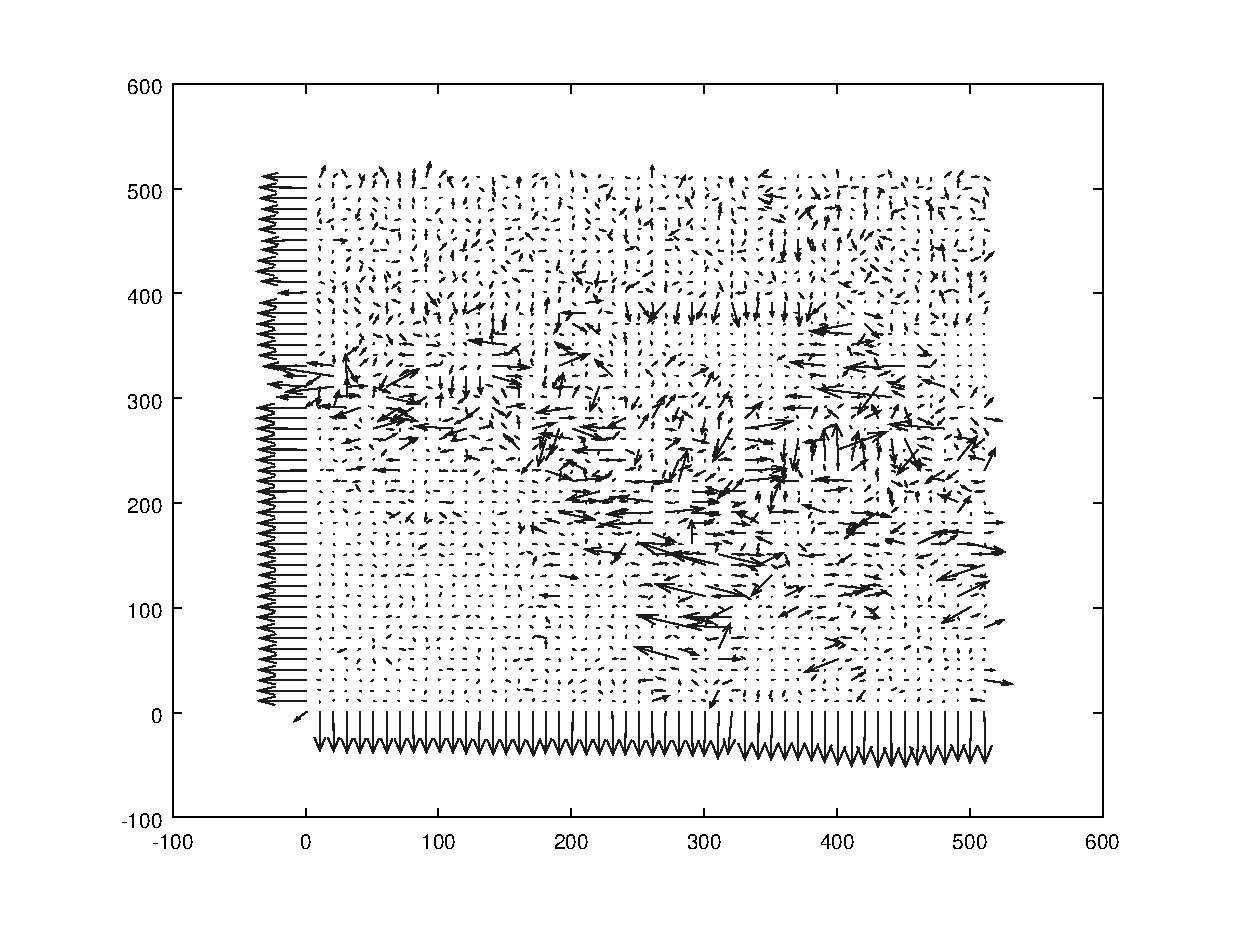
\includegraphics[height=2.5in]{./Graphics/scimmiafrecce}}
\end{tabular}
\caption{Grayscale, single-channel image (top) on which the Sobel operator $G$
has been applied. Resulting absolute value (left) and vector field
(right).\label{fig:scimmia}}
\end{figure}

\subsection{Fast normal computation from depth images} \label{sec:linemod-depth}

\subsection{Gradient quantization and binary representation of templates for
fast matching} \label{sec:linemod-binary}

\subsection{Line-MOD runtime algorithm} \label{sec:linemod-usage}

